\begin{figure}[ht]
\centering
% Thesis-wide categorical color palette
% Usage: % Thesis-wide categorical color palette
% Usage: % Thesis-wide categorical color palette
% Usage: \input{figures/palette} in any figure file
%
% Muted primary colors -- print-friendly, visually distinct.
% Inspired by Cooper Union's red/blue primaries, softened for
% academic figures. Use palA-palC for data series in scatter
% plots, line charts, bar charts, etc.

\definecolor{palA}{HTML}{1F77B4}   % Tableau blue
\definecolor{palB}{HTML}{D62728}   % Tableau red
\definecolor{palC}{HTML}{2CA02C}   % Tableau green
 in any figure file
%
% Muted primary colors -- print-friendly, visually distinct.
% Inspired by Cooper Union's red/blue primaries, softened for
% academic figures. Use palA-palC for data series in scatter
% plots, line charts, bar charts, etc.

\definecolor{palA}{HTML}{1F77B4}   % Tableau blue
\definecolor{palB}{HTML}{D62728}   % Tableau red
\definecolor{palC}{HTML}{2CA02C}   % Tableau green
 in any figure file
%
% Muted primary colors -- print-friendly, visually distinct.
% Inspired by Cooper Union's red/blue primaries, softened for
% academic figures. Use palA-palC for data series in scatter
% plots, line charts, bar charts, etc.

\definecolor{palA}{HTML}{1F77B4}   % Tableau blue
\definecolor{palB}{HTML}{D62728}   % Tableau red
\definecolor{palC}{HTML}{2CA02C}   % Tableau green

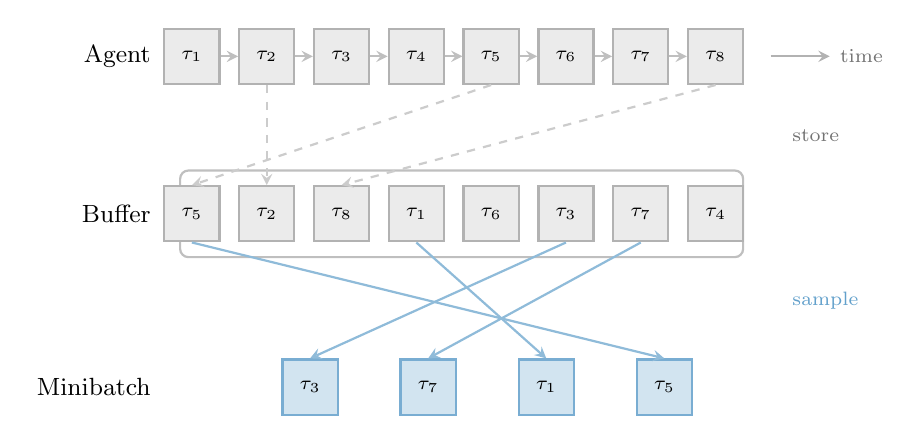
\begin{tikzpicture}[
    trans/.style={draw=black!30, thick, minimum width=0.7cm,
                  minimum height=0.7cm, font=\scriptsize,
                  inner sep=0pt, fill=black!8},
    arr/.style={->, thick, >=stealth},
    lbl/.style={font=\small},
    sublbl/.style={font=\scriptsize, text=black!55},
]

% --- Timeline (top) ---
\node[lbl, anchor=east] at (-0.4, 0) {Agent};
\node[trans] (t1) at (0, 0)    {$\tau_{1}$};
\node[trans] (t2) at (0.95, 0) {$\tau_{2}$};
\node[trans] (t3) at (1.90, 0) {$\tau_{3}$};
\node[trans] (t4) at (2.85, 0) {$\tau_{4}$};
\node[trans] (t5) at (3.80, 0) {$\tau_{5}$};
\node[trans] (t6) at (4.75, 0) {$\tau_{6}$};
\node[trans] (t7) at (5.70, 0) {$\tau_{7}$};
\node[trans] (t8) at (6.65, 0) {$\tau_{8}$};

\foreach \i in {1,...,7} {
    \pgfmathtruncatemacro{\next}{\i+1}
    \draw[arr, black!25] (t\i.east) -- (t\next.west);
}

% "time" arrow
\draw[arr, black!30] (7.35, 0) -- (8.1, 0)
    node[right, sublbl] {time};

% --- Buffer (middle) ---
\node[lbl, anchor=east] at (-0.4, -2) {Buffer};

% Buffer outline
\draw[thick, black!25, rounded corners=3pt]
    (-0.15, -2.55) rectangle (7.0, -1.45);

% Transitions in buffer (shuffled order)
\node[trans] (b5) at (0, -2)    {$\tau_{5}$};
\node[trans] (b2) at (0.95, -2) {$\tau_{2}$};
\node[trans] (b8) at (1.90, -2) {$\tau_{8}$};
\node[trans] (b1) at (2.85, -2) {$\tau_{1}$};
\node[trans] (b6) at (3.80, -2) {$\tau_{6}$};
\node[trans] (b3) at (4.75, -2) {$\tau_{3}$};
\node[trans] (b7) at (5.70, -2) {$\tau_{7}$};
\node[trans] (b4) at (6.65, -2) {$\tau_{4}$};

% Store arrows (a few representative ones)
\draw[arr, black!20, dashed] (t2.south) -- (b2.north);
\draw[arr, black!20, dashed] (t5.south) -- (b5.north);
\draw[arr, black!20, dashed] (t8.south) -- (b8.north);
\node[sublbl, right] at (7.5, -1.0) {store};

% --- Minibatch (bottom) ---
\node[lbl, anchor=east] at (-0.4, -4.2) {Minibatch};

% Sampled transitions (non-consecutive)
\node[trans, fill=palA!20, draw=palA!60]
    (m1) at (1.5, -4.2) {$\tau_{3}$};
\node[trans, fill=palA!20, draw=palA!60]
    (m2) at (3.0, -4.2) {$\tau_{7}$};
\node[trans, fill=palA!20, draw=palA!60]
    (m3) at (4.5, -4.2) {$\tau_{1}$};
\node[trans, fill=palA!20, draw=palA!60]
    (m4) at (6.0, -4.2) {$\tau_{5}$};

% Sample arrows
\draw[arr, palA!50] (b3.south) -- (m1.north);
\draw[arr, palA!50] (b7.south) -- (m2.north);
\draw[arr, palA!50] (b1.south) -- (m3.north);
\draw[arr, palA!50] (b5.south) -- (m4.north);
\node[sublbl, right, text=palA!70] at (7.5, -3.1) {sample};

\end{tikzpicture}
\caption{Experience replay. Transitions arrive sequentially and are
  stored in a buffer. Training minibatches are sampled randomly,
  breaking the temporal correlations.}
\label{fig:replay-buffer}
\end{figure}
